\documentclass[12pt]{article}
\usepackage[a4paper,margin=1.25cm]{geometry}
\usepackage{amsmath,amssymb,mathtools}
\usepackage{graphicx}
\usepackage{booktabs}
\usepackage{tabularx}
\usepackage{tikz}
\usepackage[T1]{fontenc}
\usepackage[utf8]{inputenc}
\usepackage[english]{babel}

\setlength{\parindent}{0pt}
\setlength{\parskip}{0.45em}
\setlength{\abovedisplayskip}{5pt plus 1pt minus 1pt}
\setlength{\belowdisplayskip}{5pt plus 1pt minus 1pt}
\setlength{\abovedisplayshortskip}{3pt plus 1pt minus 1pt}
\setlength{\belowdisplayshortskip}{3pt plus 1pt minus 1pt}

\newcommand{\dd}{\,\mathrm{d}}
\newcommand{\ii}{\mathrm{i}}
\newcommand{\e}{\mathrm{e}}
\newcommand{\Log}{\operatorname{Log}}
\newcommand{\Arg}{\operatorname{Arg}}
\newcommand{\res}{\operatorname*{Res}}
\newcommand{\PV}{\operatorname{PV}}
\newcommand{\Rp}{\operatorname{Re}}
\newcommand{\Ip}{\operatorname{Im}}
\newcommand{\Int}{\operatorname{Int}}

\begin{document}

\begin{center}
{\Large\bfseries A log-cosine integral and a pole on the contour}\\[0.35em]
{\large the hidden circle \(\left|u-\tfrac12\right|=\tfrac12\) and the half-residue at \(u=1\)}
\end{center}

\[
\boxed{\displaystyle
\int_0^{\pi/2}
\frac{\log\cos x}{x^2+\log^2\cos x}\dd x
=\frac{\pi}{2}\left(1-\frac1{\log2}\right).}
\]

\textbf{Overview.}
The quadratic form \(x^2+\log^2\cos x\) in the denominator is the squared
modulus of the complex number
\[
w(x)=\log\cos x+\ii x,
\]
and the numerator is its real part, so the integrand is
\(\Rp\frac1{w(x)}\). Exponentiating,
\[
u=\e^{w(x)}=\cos x\,\e^{\ii x}=\frac{1+\e^{2\ii x}}{2},
\]
which is a circle of radius \(\frac12\) centred at \(\frac12\), traversed
once as \(x\) runs over \((-\frac\pi2,\frac\pi2)\). The integral therefore
becomes a contour integral of
\[
H(u)=\frac1{\left(u-\frac12\right)\Log u}
\]
around that circle. Two singular points matter: an interior pole at
\(u=\frac12\), the centre, which produces the term \(-\frac{\pi}{2\log2}\),
and a pole \emph{on} the contour at \(u=1\), which produces the term
\(\frac\pi2\) through the half-residue rule. The endpoint \(u=0\), where
\(\log\cos x\) blows up, contributes nothing.

The tangency structure here is the mirror image of the \(\log\sin\) case:
there the circle is \(|u-\frac{\ii}2|=\frac12\) and the mean-value
property applies cleanly; here the circle is \(|u-\frac12|=\frac12\) and
a pole sits on it, so the mean-value property must be replaced by a
principal-value residue computation.

\section*{1. The hidden complex variable}

Set
\[
w(x)=\log\cos x+\ii x,\qquad -\frac\pi2<x<\frac\pi2 .
\]
Then
\[
\frac1{w(x)}=\frac{\overline{w(x)}}{|w(x)|^2}
=\frac{\log\cos x-\ii x}{\log^2\cos x+x^2},
\]
so the integrand of the problem is exactly
\[
\Rp\frac1{w(x)}=\frac{\log\cos x}{x^2+\log^2\cos x}.
\tag{1}
\]
Since \(\cos\) is even, \(w(-x)=\overline{w(x)}\), hence
\(\frac1{w(-x)}=\overline{\frac1{w(x)}}\), and the imaginary parts cancel
on a symmetric interval:
\[
J:=\PV_{x=0}\int_{-\pi/2}^{\pi/2}\frac{\dd x}{w(x)}
=2\int_0^{\pi/2}\Rp\frac1{w(x)}\dd x
=2I .
\tag{2}
\]

\textbf{Why a principal value, and why only for \(J\).}
At \(x=0\) we have \(w(0)=0\), so \(1/w\) is singular there. Expanding,
\[
w(x)=\ii x-\frac{x^2}{2}+O(x^4),
\qquad
\frac1{w(x)}=-\frac{\ii}{x}+\frac12+O(x),
\]
so the singular part is purely imaginary and odd; the principal value at
\(x=0\) exists and kills it. The real part is bounded:
\[
\Rp\frac1{w(x)}\longrightarrow-\frac12,\qquad x\to0,
\]
so the original integral \(I\) converges as an ordinary integral. At the
other endpoint \(x\to\frac\pi2\), \(\log\cos x\to-\infty\) and the
integrand behaves like \(1/\log\cos x\to0\). Both endpoints are harmless
for \(I\).

\section*{2. Exponentiating: the circle \(|u-\frac12|=\frac12\)}

Put \(u=\e^{w(x)}\). Then
\[
u=\cos x\,\e^{\ii x}
=\frac{\e^{-\ii x}+\e^{\ii x}}{2}\,\e^{\ii x}
=\frac{1+\e^{2\ii x}}{2},
\]
that is,
\[
\boxed{\displaystyle u-\frac12=\frac12\e^{2\ii x}.}
\tag{3}
\]
As \(x\) runs from \(-\frac\pi2\) to \(\frac\pi2\), the angle \(2x\) runs
from \(-\pi\) to \(\pi\), so \(u\) traverses
\[
C:\quad\left|u-\frac12\right|=\frac12
\]
exactly once, positively oriented. The circle passes through \(u=0\) (at
\(x=\pm\frac\pi2\)) and \(u=1\) (at \(x=0\)).

\begin{center}
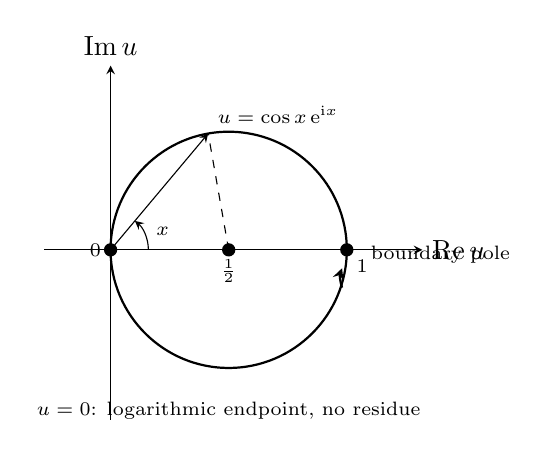
\begin{tikzpicture}[scale=3,>=stealth]
\draw[->] (-0.28,0)--(1.32,0) node[right] {\(\Rp u\)};
\draw[->] (0,-0.72)--(0,0.78) node[above] {\(\Ip u\)};
\draw[thick] (0.5,0) circle (0.5);
\fill (0,0) circle (0.8pt) node[left] {\scriptsize \(0\)};
\fill (1,0) circle (0.8pt) node[below right] {\scriptsize \(1\)};
\fill (0.5,0) circle (0.8pt) node[below] {\scriptsize \(\tfrac12\)};
\def\x{50}
\coordinate (P) at ({0.5+0.5*cos(2*\x)},{0.5*sin(2*\x)});
\draw[->] (0,0)--(P);
\node[above right] at (P) {\scriptsize \(u=\cos x\,\e^{\ii x}\)};
\draw[dashed] (0.5,0)--(P);
\draw[->] (0.16,0) arc (0:\x:0.16);
\node at (0.22,0.08) {\scriptsize \(x\)};
\draw[->,thick] (0.98,-0.16) arc (200:160:0.12);
\node[right] at (1.06,-0.02) {\scriptsize boundary pole};
\node at (0.5,-0.68) {\scriptsize \(u=0\): logarithmic endpoint, no residue};
\end{tikzpicture}
\end{center}

The branch is fixed by the geometry: every point of \(C\) except \(u=0\)
has \(\Rp u>0\), so the correct logarithm is the principal one restricted
to the right half-plane,
\[
\Log u=\log|u|+\ii\Arg u,\qquad -\frac\pi2<\Arg u<\frac\pi2,
\]
and with this choice \(w(x)=\Log u\) identically, since
\(\Ip w=x\in(-\frac\pi2,\frac\pi2)\).

Differentiating (3),
\[
\dd u=\ii\e^{2\ii x}\dd x=2\ii\left(u-\frac12\right)\dd x,
\qquad
\dd x=\frac{\dd u}{2\ii\left(u-\frac12\right)}.
\tag{4}
\]
Substituting (4) into (2),
\[
J=\frac1{2\ii}\PV\int_C
\frac{\dd u}{\left(u-\frac12\right)\Log u}
=\frac1{2\ii}\PV\int_C H(u)\dd u,
\qquad
H(u)=\frac1{\left(u-\frac12\right)\Log u}.
\tag{5}
\]

\section*{3. The three special points of \(H\) on and inside \(C\)}

\textbf{(a) \(u=\frac12\), interior, simple pole.} The centre of the
circle is inside \(C\) and \(\Log\frac12=-\log2\ne0\), so
\[
\res_{u=1/2}H=\frac1{\Log\frac12}=-\frac1{\log2}.
\tag{6}
\]

\textbf{(b) \(u=1\), on the contour, simple pole.} Here \(\Log u\)
vanishes to first order: \(\Log u=(u-1)-\frac{(u-1)^2}{2}+\cdots\). Hence
\(H\) has a simple pole at \(u=1\) with
\[
\res_{u=1}H
=\lim_{u\to1}\frac{u-1}{\left(u-\frac12\right)\Log u}
=\frac1{\frac12}
=2 .
\tag{7}
\]
This is the point \(x=0\), the same singularity for which the principal
value was introduced in Section 1.

\textbf{(c) \(u=0\), on the contour, not a pole.} Although \(\Log u\)
is singular at the origin, \(H\) is not: \(\frac1{\Log u}\to0\) as
\(u\to0\). If the contour is indented by a small arc of radius
\(\varepsilon\) at the origin, the contribution is bounded by
\[
\frac{C\varepsilon}{|\log\varepsilon|}\longrightarrow0 ,
\]
since the arclength is \(O(\varepsilon)\), the factor
\(\left(u-\frac12\right)^{-1}\) is bounded there, and
\(|\Log u|\ge|\log\varepsilon|\). So the origin may be ignored.

\section*{4. Principal value with a pole on the contour}

\textbf{Lemma (half-residue).}
Let \(C\) be a positively oriented smooth closed contour, and let \(H\)
be holomorphic near \(C\) and inside it except for finitely many poles,
those on \(C\) being simple. Then
\[
\boxed{\displaystyle
\PV\int_C H(u)\dd u
=2\pi\ii\sum_{a\in\Int C}\res_{u=a}H
+\ii\pi\sum_{a\in C}\res_{u=a}H .}
\tag{8}
\]

\textit{Sketch.} Indent \(C\) at each boundary pole \(a\) by a small
circular arc of radius \(\varepsilon\) pushed outside the region. The
indented contour encloses only the interior poles, giving the first sum.
A simple pole with residue \(r\) contributes, over an arc of opening
angle \(\pi\) (the tangent line, in the limit \(\varepsilon\to0\)),
\[
\int_{\text{arc}}\frac{r}{u-a}\dd u
=r\,\ii\!\int\!\dd\varphi=\ii\pi r
\]
with sign fixed by the orientation, and the remaining regular part of
\(H\) contributes \(O(\varepsilon)\). Passing to the limit gives (8).
\(\square\)

The geometric reading is that a pole sitting on a smooth boundary is
``half inside'', so it enters with half its usual weight
\(2\pi\ii\to\ii\pi\).

\begin{center}
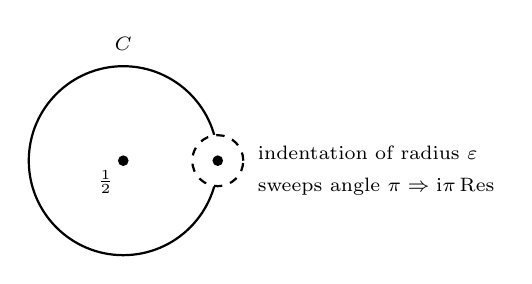
\begin{tikzpicture}[scale=2.4,>=stealth]
\draw[thick] (0.5,0) circle (0.5);
\filldraw[fill=white,draw=white] (1,0) circle (0.135);
\draw[thick,dashed] (1,0) circle (0.135);
\draw[thick] (0.5,0)+(0:0) circle (0);
\fill (1,0) circle (0.8pt);
\node[right] at (1.16,0.04) {\scriptsize indentation of radius \(\varepsilon\)};
\node[right] at (1.16,-0.14) {\scriptsize sweeps angle \(\pi\Rightarrow\ii\pi\,\mathrm{Res}\)};
\fill (0.5,0) circle (0.8pt) node[below left] {\scriptsize \(\tfrac12\)};
\node at (0.5,0.62) {\scriptsize \(C\)};
\end{tikzpicture}
\end{center}

\section*{5. Evaluation}

Applying (8) with the residues (6) and (7), and with the origin excluded
by Section 3(c),
\[
\PV\int_C H(u)\dd u
=2\pi\ii\left(-\frac1{\log2}\right)+\ii\pi\cdot2
=2\pi\ii\left(1-\frac1{\log2}\right).
\]
By (5),
\[
J=\frac1{2\ii}\cdot 2\pi\ii\left(1-\frac1{\log2}\right)
=\pi\left(1-\frac1{\log2}\right),
\]
and by (2), \(I=\frac J2\):
\[
\boxed{\displaystyle
\int_0^{\pi/2}
\frac{\log\cos x}{x^2+\log^2\cos x}\dd x
=\frac\pi2\left(1-\frac1{\log2}\right)
=-0.69538374\ldots}
\]
The sign is a useful check: \(\log\cos x<0\) on \((0,\frac\pi2)\), so the
integrand is negative throughout, and indeed \(\frac1{\log2}>1\).
Numerical quadrature gives \(-0.6953837441187\ldots\), agreeing to all
displayed digits.

\section*{6. The anatomy of the answer}

The two terms of the result come from two geometrically distinct sources,
and it is worth separating them.

\begin{center}
\small
\renewcommand{\arraystretch}{1.45}
\begin{tabularx}{\textwidth}{@{}>{\raggedright\arraybackslash}p{0.16\textwidth}>{\raggedright\arraybackslash}p{0.20\textwidth}>{\raggedright\arraybackslash}p{0.16\textwidth}X@{}}
\toprule
Point & Nature & Contribution to \(I\) & Source \\
\midrule
\(u=\tfrac12\) & interior simple pole & \(-\dfrac{\pi}{2\log2}\) &
The centre of the circle: this is the mean-value term, the analogue of
\(\pi F(w_0)\). \\
\addlinespace
\(u=1\) & simple pole on \(C\) & \(+\dfrac{\pi}{2}\) &
The point \(x=0\), where \(w(0)=0\); a half-residue. \\
\addlinespace
\(u=0\) & logarithmic endpoint & \(0\) &
\(1/\Log u\to0\) faster than the arclength shrinks. \\
\bottomrule
\end{tabularx}
\end{center}

Written as \(I=\frac\pi2-\frac{\pi}{2\log2}\), the first term is pure
boundary geometry and carries no arithmetic constant, whereas the
\(\log2\) is the value \(\Log\frac12\) at the centre of the circle. This
is why \(\log 2\) appears in a problem whose statement mentions no
logarithm of a constant: \(\frac12\) is the centre of the hidden circle.

\section*{7. Comparison with the mean-value case}

For the \(\log\sin\) family one has \(u=\sin x\,\e^{\ii x}\), the circle
\(\left|u-\frac{\ii}2\right|=\frac12\) tangent to the origin, and for
holomorphic \(F\) the clean identity
\[
\int_0^\pi F(\log\sin x+\ii x)\dd x=\pi F\!\left(\Log\frac{\ii}{2}\right),
\]
the mean-value property transported by \(u\mapsto\Log u\). The temptation
is to write the present problem the same way with \(F(w)=1/w\) and
conclude \(\int\frac{\dd x}{w}=\pi/w_0\) with \(w_0=\Log\frac12=-\log2\),
giving \(-\frac{\pi}{\log2}\) for \(J\), which is wrong by exactly
\(\pi\).

The discrepancy is the whole content of the problem: \(F(w)=1/w\) is
\emph{not} holomorphic on the closed region, because \(w_0=0\) is
attained on the boundary curve at \(x=0\). In \(u\) coordinates that is
the pole of \(H\) at \(u=1\in C\). The mean-value property applies to the
regular part and yields \(-\frac{\pi}{\log 2}\); the half-residue at the
boundary pole restores the missing \(+\pi\).

\begin{center}
\small
\renewcommand{\arraystretch}{1.4}
\begin{tabularx}{0.94\textwidth}{@{}>{\raggedright\arraybackslash}p{0.30\textwidth}XX@{}}
\toprule
& \(\log\sin\) family & this problem \\
\midrule
Curve
& \(u=\sin x\,\e^{\ii x}\)
& \(u=\cos x\,\e^{\ii x}\) \\
Circle
& \(\left|u-\frac{\ii}2\right|=\frac12\)
& \(\left|u-\frac12\right|=\frac12\) \\
Branch strip
& \(0<\Ip w<\pi\)
& \(|\Ip w|<\frac\pi2\) \\
Centre
& \(w_0=-\log2+\frac{\pi\ii}{2}\)
& \(w_0=-\log2\) \\
Obstruction
& none for \(F=\Log\Log\)
& \(F=1/w\) has a pole at \(w_0'=0\in\partial\) \\
Result
& \(\pi F(w_0)\)
& \(\pi F(w_0)+\ii\pi\cdot\frac1{2\ii}\res\) \\
\bottomrule
\end{tabularx}
\end{center}

\section*{8. Variants that come free}

Once (5) is set up, other integrands are simply other \(H\).

\textbf{The imaginary part.} Taking \(-\Ip\frac1w\) instead of
\(\Rp\frac1w\) gives an odd integrand, so
\[
\int_0^{\pi/2}\frac{x}{x^2+\log^2\cos x}\dd x
\]
is \emph{not} obtained by this symmetry argument. It corresponds to
the divergent part removed by the principal value, and indeed diverges
logarithmically at \(x=0\), where the integrand behaves like \(1/x\).

\textbf{Shifted denominators.} For real \(a>0\), replace \(w\) by
\(w+a\), i.e. take
\[
H_a(u)=\frac1{\left(u-\frac12\right)(\Log u+a)} .
\]
The zero of \(\Log u+a\) is \(u=\e^{-a}\in(0,1)\), which satisfies
\(\left|\e^{-a}-\frac12\right|<\frac12\) and hence lies strictly
\emph{inside} \(C\). So for \(a>0\) there is no pole on the contour, (8)
reduces to the ordinary residue theorem with the two interior poles
\(u=\frac12\) and \(u=\e^{-a}\), and
\[
\res_{u=1/2}H_a=\frac1{a-\log2},
\qquad
\res_{u=\e^{-a}}H_a
=\frac{1}{\left(u-\frac12\right)\frac1u}\bigg|_{u=\e^{-a}}
=\frac{\e^{-a}}{\e^{-a}-\frac12}.
\]
This gives, for every \(a>0\),
\[
\boxed{\displaystyle
\int_0^{\pi/2}\frac{\log\cos x+a}{(\log\cos x+a)^2+x^2}\dd x
=\frac\pi2\left[\frac1{a-\log2}
+\frac{\e^{-a}}{\e^{-a}-\frac12}\right].}
\tag{9}
\]

Formula (9) is discontinuous at \(a=0\). Letting
\(a\to0^+\) in (9),
\[
\frac\pi2\left[-\frac1{\log2}+\frac{1}{1-\frac12}\right]
=\frac\pi2\left(2-\frac1{\log2}\right),
\]
whereas the value at \(a=0\) computed in Section 5 is
\(\frac\pi2\bigl(1-\frac1{\log2}\bigr)\). The jump is exactly \(\frac\pi2\),
half the interior contribution of the pole that is crossing the contour.

The same jump is visible on the real side without any complex analysis.
Near \(x=0\) we have \(\log\cos x=-\frac{x^2}{2}+O(x^4)\), so for small
\(a>0\) the integrand of (9) is approximately \(\frac{a}{a^2+x^2}\),
whose integral over a fixed neighbourhood of \(0\) is
\(\arctan\frac{\delta}{a}\to\frac\pi2\). A spike of height \(1/a\) and
width \(a\) carries a fixed mass \(\frac\pi2\) and disappears at \(a=0\),
where the integrand is merely bounded, tending to \(-\frac12\). The
half-residue rule of Section 4 is the complex-analytic bookkeeping for
precisely this Poisson-kernel spike.

\end{document}
